\documentclass[11pt]{article}
\usepackage{incgraph, tikz, csquotes, float}

\newcommand{\attachment}[1]{
	\incgraph[label={#1},overlay page number at bottom][scale=0.5]{pictures/#1.png}
}

\newcommand{\attachmentpdf}[1]{
	\incgraph[label={#1},overlay page number at bottom][scale=0.5]{pictures/#1.pdf}
}

\begin{document}
	\title{Software Reengineering Project}
	\author{Mitchel Pyl \& Randy Paredis}
	\date{}
	
	\maketitle
	
	\section{Introduction}
	This document is meant as additional information on the reengineering and refactoring of the \texttt{JFreeChart} project, which was the assignment of the \textsf{Software Reengineering} course of 2019, at the \textsf{University of Antwerp}.
	
	During this paper and the process of reengineering the \texttt{JFreeChart} project, we relied heavily on \cite{demeyer2009object}, making sure we could complete our assignment as successful as possible.
	
	\texttt{JFreeChart} \cite{jfreechart} is a Java library that can be used to add/show professional-looking graphs and charts in your Java applications. This inheritly implies that is it useful in a lot of different contexts and scenarios that require this kind of feature.
	
	The ability for such a library for being flexible and expandable with a vast amount of new features would therefore be an incredible advantage for this.
	
	\subsection{Problem at Hand}
	\label{sec:pah}
	At this point in time, \texttt{JFreeChart} has a wide range of possible graphs, charts and plots it can generate for any kind of data you'd like. However, there is some functionality missing that we'd like to have. Namely, we'd like to be able to have a different shape or symbol for each datapoint. In order for us to introduce this feature, we'll first have to figure out the current way rendering of datapoints is handeled and afterwards we'll refactor the code so we can easily add this feature.
	
	Additionally, when we take a closer look at the code in general, there are some symptoms indicating it should be refactored\footnote{\textit{Missing tests}, \textit{Too much time for simple changes}...; 1.1 from \cite{demeyer2009object})}.
	
	\section{Project Management}
	\subsection{Setting Direction}
	The most important aspect of managing a reengineering project is to find a strategy in which the reengineering will be the most useful and succesful (Chapter 2 from \cite{demeyer2009object}). This is why we first discussed a strategy to use in the actual reengineering, before jumping into the code like headless chickens.
	
	Using some tools, we were able to \textsl{Agree on Maxims} (2.1 from \cite{demeyer2009object}) and more specifically the \textsl{Most Valuable First} (2.4 from \cite{demeyer2009object}). With these strategies in mind, we can give all refactoring targets a weight, so we can easily list the most important ones. As described in 2.4 from \cite{demeyer2009object}, such a weight technically has nothing to do with cyclic complexities, but with what's valuable to the customer. In our case, these luckily (or coincidentally) line up to a certain point.
	
	Learning the most important rule in software reengineering,
	\textsl{If It Ain't Broke, Don't Fix It.} (2.6 from \cite{demeyer2009object})\footnote{Note: this is a rule, not a lifeline, nor an excuse. (as per \cite{demeyer2009object})}, we know we'd best not touch any code that is "working" correctly and has nothing to do with any of the valuable targets. For instance, within the scope of the assignment, it is not useful to take a look at refactoring the \texttt{ImageMapUtils}.
	
	While on the topic, although all strategies have their merit and are important in some way, we believe some of them are more important and/or practical to follow. \textsl{Keep It Simple} (2.7 from \cite{demeyer2009object}) is one of them, which we will keep in mind during the refactoring process.
	
	\subsection{Original Idea}
	\label{sec:original}
	Not all planning processes will happen as they were imagined. In our original report, we showed a simplified \textsf{PERT} chart, on which we would base ourselves in the refactoring process. Unfortunately, as we will mention in \textsl{section \ref{sec:management2}}, our original concept was turned upside-down.
	
	\subsubsection{PERT Chart} 
	\begin{figure}[H] 
		\centering 
		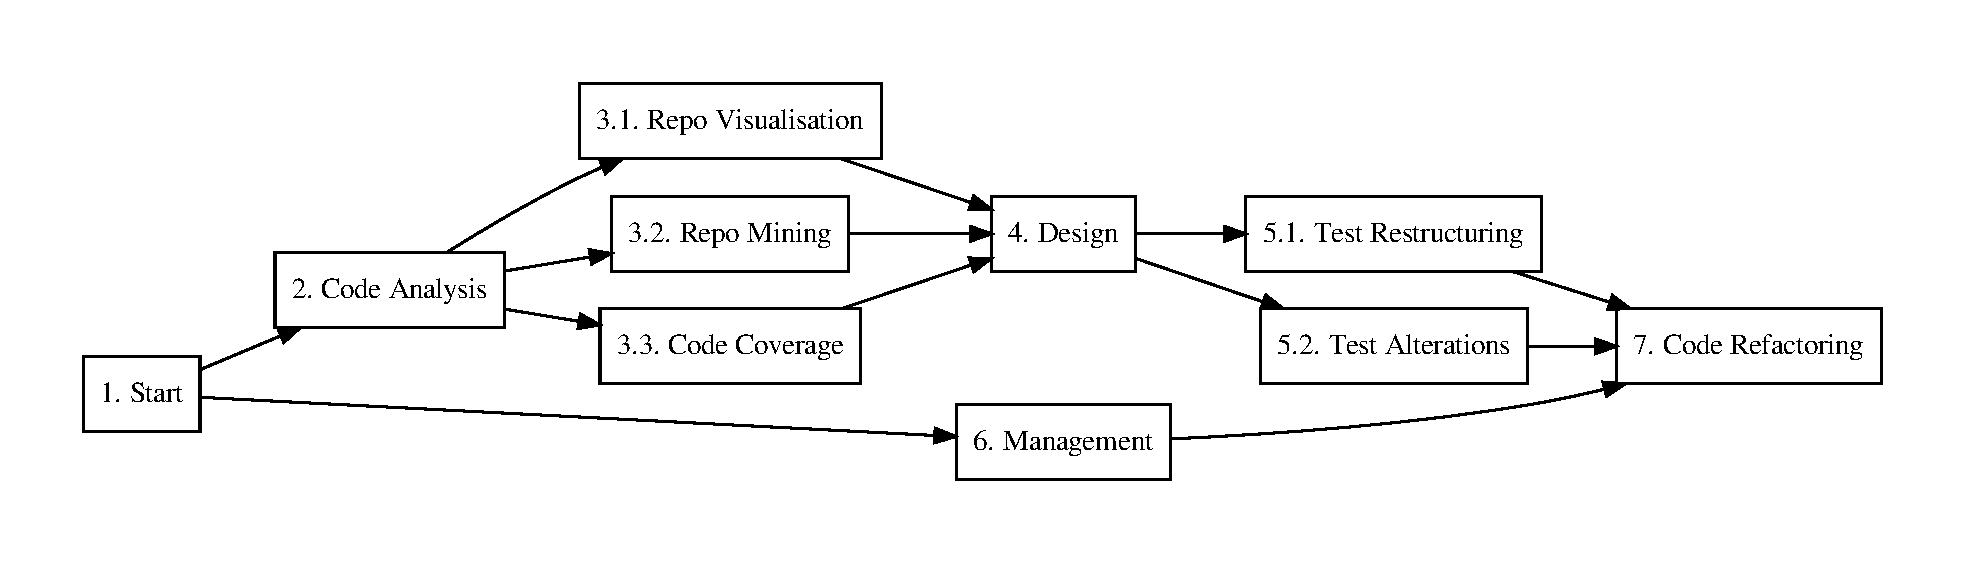
\includegraphics[width=\textwidth]{pictures/pert-original.pdf}
		\caption{Original simplified \textsf{PERT} chart idea for the Refactoring of \texttt{JFreeChart}.} 
		\label{fig:pert-orig} 
	\end{figure} 
   
	In order for us to cleanly work on the reengineering of \texttt{JFreeChart}, we decided to make a \textsf{PERT} chart \cite{pert}, as you can see in \textsl{Fig.\,\ref{fig:pert-orig}}. This is a simplified model, without annotations of any critical tasks, paths, or the latest end dates for each task. 
   
	As you can see, \textsl{Management} is a task we will do throughout the entire process of refactoring the project. Tasks \textsl{3.1. Repo Visualisation}, \textsl{3.2 Repo Mining} and \textsl{3.3 Code Coverage} can be found later in this document, respectively in \textsl{sections \ref{sec:gource}, \ref{sec:codescene}} and \textsl{\ref{sec:coco}}.
	
	\subsubsection{Gantt Chart}
	To accommodate for our original \textsf{PERT} chart, we decided to add a \textsf{Gantt} chart \cite{gantt} with our guesses on timing constraints.
	
	\begin{figure}[H] 
		\centering 
		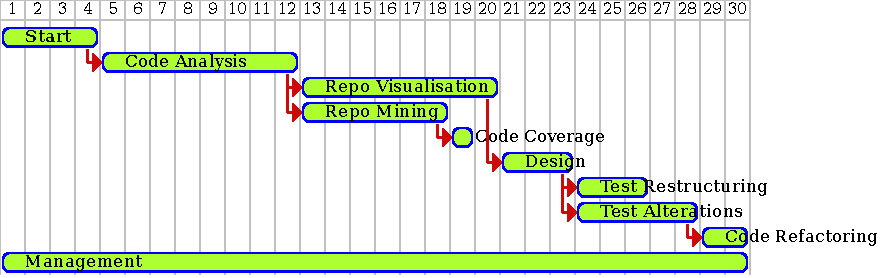
\includegraphics[width=\textwidth]{pictures/gantt-original.pdf}
		\caption{Original \textsf{Gantt} chart idea for the Refactoring of \texttt{JFreeChart}. Image made with \cite{plantuml}.} 
		\label{fig:gantt-orig} 
	\end{figure} 

	As you can see in the chart above, all tasks that appear in the \textsf{PERT} chart are listed here, with an approximation of how long we believe these should take and when we should start working on them.
   
	
	\subsection{First Contact}
	Seeing as we don't have any experience with the project, nor with its uses, we tried to get a good, general overview. When trying to \textsl{Read all the Code in One Hour} (3.2 from \cite{demeyer2009object}) and to \textsl{Skim the Documentation} (3.3 from \cite{demeyer2009object}), we found that is was quite the difficult task and although it certainly helped in getting a good understanding of how the system worked, it was far from ideal.
	
	
	\section{Project Analysis and Tool Usage}
	In order to solidly identify the issues with \texttt{JFreeChart} and find possible refactoring targets, we made use of a few helpful tools that allowed for clear identification of possible problem areas. This way we can clearly \textsl{Study the Exceptional Entities} (4.3 from \cite{demeyer2009object}). Even though we know that what we find may be tedious or ambiguous to interpret, we will still make our conclusions based on what we know and expect.
	
	In general, we used both \textsf{IntelliJ} \cite{intellij} and \textsf{Ecipse} \cite{eclipse} for analyzing and browsing through our project. Both IDEs have easy functionalities to allow for refactoring, but our main process was done using \textsf{IntelliJ}, with additional analysis in \textsf{Eclipse}.
	
	\subsection{Repository Visualization with Gource}
	\label{sec:gource}
	The first tool we made use of was \textsf{Gource} \cite{gource}. It is a clean and fancy piece of software that can turn the history of a git repository into a visual representation. This is useful for a few reasons. First, it allows us to see clearly who the main contributers are. There was no surprise that this was \textsl{David Gilbert}.
	
	A second thing we could deduce from this simulation is that the code was not made using the \textsf{Test Driven Development} methodology. We can clearly see that there are first adaptations to the codebase, before changing the tests.
	
	Thirdly, we can identify the possible points in time when a refactoring stage happened in this project. These are moments when a lot of files are added, removed, or modified; which is highlighted in \textsf{Gource}. Granted, it is possible that some of these changes are due to merging multiple branches together.
	
	We've identified that possible refactorings happened in November 2008 (increase in functionality), March 2013 (update to almost all files), December 2014 (update to almost all files and removal of a lot of files), July 2017 (file tree restructuring) and July 2018 (general changes).
	
	Finally, we can use the resulting visualization to \textsl{Learn from the Past} (5.5 from \cite{demeyer2009object}). We can see which classes were changed a lot and which ones remained untouched for the main bulk of the development.
	
	Classes that changed a lot most likely indicate that they are coupled to other classes in the system, marking these classes as important in understanding the general feel of the system.
	
	Classes that remained mainly untouched could indicate abandoned code, but let's assume another possibility. Let's say that these classes indicate features or functionality that are complete. Usually these features cannot give a good enough representation of what's important in the system and whatnot. In either case of untouched code, we can remove our focus from these classes.
	
	As much as we want to add screenshots to explain our findings better, \textsf{Gource} makes a video of the history of a repository. We don't want to cloud our document by adding each frame as a screenshot.
	
	\subsection{Repository Mining with CodeScene}
	\label{sec:codescene}
	Another tool we made use of was \textsf{CodeScene} \cite{codescene}, the powerful visualization tool using \textit{Predictive Analytics} to find hidden risks and social patterns in your code.
	
	\textsf{CodeScene} allowed us to get a general feel of the current state of \texttt{JFreeChart}. It gave us a clear representation of possible refactoring targets (see \textsl{attachment \pageref{refactoring-overview}}) and hotspots (see \textsl{attachment \pageref{hotspots-overview}}) within the code\footnote{Please refer to the attachments at the end of this document.}.
	
	When we take a deeper look into the code (or at least the graphical representation thereof), we can identify that we most probably will need to take a look at the \texttt{org.jfree.chart.renderer} package (see \textsl{attachment \pageref{hotspots-package-renderer}}) and the \texttt{org.jfree.chart.plot} package (see \textsl{attachment \pageref{hotspots-package-plot}}), as far as the hotspots are concerned.
	
	On the topic of refactoring targets, it is clear that the \texttt{org.jfree.chart.plot} package (see \textsl{attachment \pageref{refactoring-package-plot}}) really inquires our attention. More specifically the \texttt{XYPlot} (\textsl{attachment \pageref{refactoring-XYPlot}}), \texttt{CategoryPlot} (\textsl{attachment \pageref{refactoring-CategoryPlot}}), \texttt{PiePlot} (\textsl{attachment \pageref{refactoring-PiePlot}}), \texttt{AbstractXYItemRenderer} (\textsl{attachment \pageref{refactoring-AbstractXYItemRenderer}}) and\\ \texttt{AbstractCategoryItemRenderer} (\textsl{attachment \pageref{refactoring-AbstractCategoryItemRenderer}}) classes. In the attachments, the most complex functions are listed (sorted from high to low complexity). These top functions\footnote{The ones with a red cyclomatic complexity.} are most likely to be refactoring targets.
	
	\subsection{Code Coverage with Cobertura}
	\label{sec:coco}
	Chapter 6.3 of \cite{demeyer2009object} tells us to \textsl{Use a Testing Framework}. Not only is this a good idea in refactoring, but in all software projects in general. JUnit was already available in \texttt{JFreeChart}, so there is no need to change of alter this part of the project. Linked with JUnit was \textsf{Cobertura} \cite{cobertura}, a maven plugin that allows us to check how much code was covered with the available tests.
	
	The overview that is generated from this plugin (see \textsl{attachment \pageref{cobertura-begin}}) gives us enough information in order to determine which classes and functions were not covered in the project, also yielding possible missing tests. These missing tests can be seen as a symptom for code requiring refactoring (1.1 from \cite{demeyer2009object}). But as discussed above, we will \textsl{Fix Problems, Not Symptoms} (2.5 from \cite{demeyer2009object}) and more specifically, we will mainly focus on the tests that concern our main refactoring targets.
	
	In general, we can deduce that the code coverage of \texttt{JFreeChart} at this point in time is way below comfortable for us.
	
	We also noticed that there is currently no mutation testing being done on this project. Even though we do realize this would give way too much situations and possibilities to cover, we currently have no idea of how good the tests currently are.
	
	\subsection{Code Smells}
	\subsubsection{IntelliJ/Eclipse Plugins}	
	Due to our usage with \textsf{IntelliJ}, we also installed the \textsf{Code Smells Detector} plugin \cite{jetbrains-csd}. It allows refactoring of methods with a high cyclomatic complexity at their most complex statements, but unfortunately it does not take code clones in the functions themselves into a count. This is why we combined this plugin with the \textsf{CodeMetrics} plugin \cite{jetbrains-cm}, so we could obtain a valid annotation on the complexity of some functions that were highlighted by the \textsf{Code Smells Detector}. The functions we found here (mostly) lined up with the one we obtained from \textsf{CodeScene}, giving us additional confirmation. See \textsl{attachment \pageref{intellij-plugins}} for an example of how these two plugins look combined on a section of the \texttt{RenderStateShape} class\footnote{Which is a class we created during our refactoring process.}.
	
	The \textsf{Eclipse} counterpart of this plugin would be \textsf{JDeodorant} \cite{jdeodorant}, but sadly it was quite confusing to use and the results it produced (extracting a few methods to a superclass, moving a method to the class that is used the most in that method...) were, in our opinion, not helpful whatsoever. This is why we decided to identify most of the methods that needed extracting ourselves first and checking the result again afterwards, to see if we have made a difference.
	
	\subsubsection{Code Clones with iClones}
	While on the topic of code smells, we also used \textsf{iClones} so we could detect duplicate code and other aspects outside of the IDEs we're using. But in our opinion, this software is confusing, overly complex and does not actually show clones. It has the functionality to compare different versions of a project, but we did not find how to use this.
	
	After talking to other groups, we heard that we were not the only ones that found this.
	
	\subsection{SonarQube}
	\label{sec:sonarqube}
	After the disappointment that \textsf{iClones} is, we took a look at \textsf{SonarQube} \cite{sonarqube}. It is an online resource that can easily be integrated with a \textsf{GitHub} repository. It supports a general analysis of code smells, bugs and vulnerabilities.
	
	In \textsl{attachment \pageref{sonarcloud-orig}} you can find a general overview of what \textsf{SonarQube} found of \texttt{JFreeChart} after our refactoring. As you can see, the thing that jumps out the most is the 0\% coverage of unit tests. We believe this is due to the usage of \textsf{Cobertura} instead of \textsf{JaCoCo}, which is more common.
	
	
	\section{Refactoring}
	\subsection{Design Recovery}
	In order for us to describe our proposed new design of \texttt{JFreeChart}, we must first tell you a little bit more about the original design.
	
	\texttt{JFreeChart} consisted of 658 classes, the multitude of which have nothing to do with our problem domain. When we only focus on the classes that are important (as per 2.4 and 2.6 from \cite{demeyer2009object}), we can create a UML diagram. But because the way \texttt{JFreeChart} is currently designed, the UML class diagram of the subsection we will describe is incredibly wide and messy to look at. This is why we adapted the UML specification to get a clearer picture of what is actually happening (see \textsl{Fig.\,\ref{fig:UML-start}}).
	
	\begin{figure}[H]
		\centering
		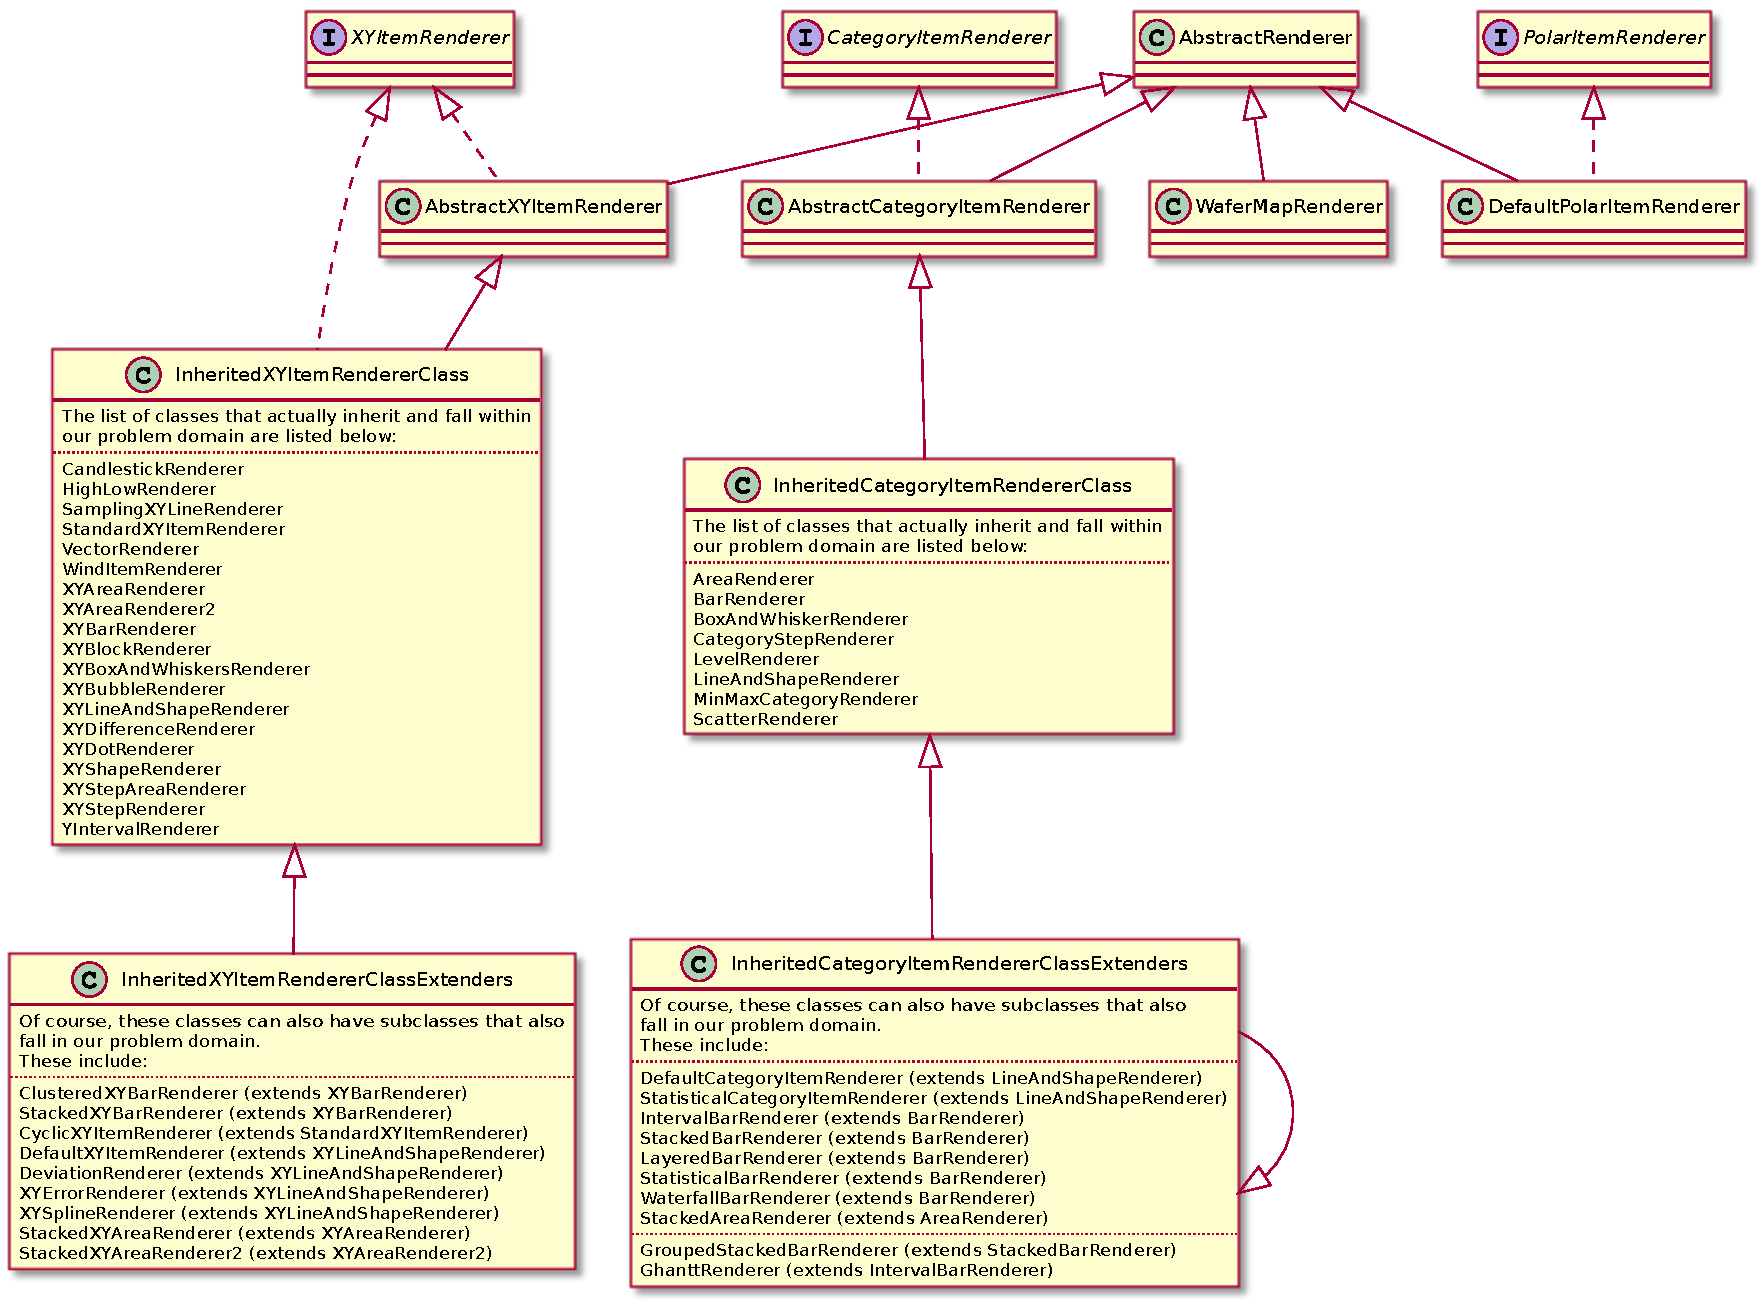
\includegraphics[width=\textwidth]{pictures/class-diagram-begin.pdf}
		\caption{A simplified representation of the UML class diagram at the beginning of the refactoring process. Image created with \cite{plantuml}. A bigger version can be found in \textsl{attachment \pageref{class-diagram-begin}}.}
		\label{fig:UML-start}
	\end{figure}
	
	The \texttt{InheritedXYItemRendererClass} in our UML class diagram represents any subclass of the \texttt{AbstractXYItemRenderer}. The same was done for the \texttt{InheritedCategoryItemRenderer} and the \texttt{AbstractCategoryItemRenderer}. In the \texttt{Extenders}, the few classes that extend from the \texttt{InheritedRenderers} are listed in the same way\footnote{Though, for the \texttt{Category} case there is another layer in the structure, hence the self-referring arrow in the \texttt{InheritedCategoryItemRendererClassExtenders}.}.
	
	This expansion of the UML specification allowed us to generally show the structure of our problem domain. Yet, trying to identify this domain, or more specifically, the functionality that required refactoring was quite tricky. This is mainly due to the high rate of exceptional entities and anomalies we've found while applying the \textsl{Study the Exceptional Entities} pattern (4.3 from \cite{demeyer2009object}).
	
	Some of these anomalies\footnote{As we would describe them. In \cite{demeyer2009object} they are not mentioned.}, we've listed below.
	\begin{itemize}
		\item Renderers that do not render;
		%\item Inconsistent usage of drawing shapes between classes that inherit from the same base. (e.g. \texttt{drawRect} and \texttt{draw(Rectange)});
		\item Implicit implementation of interfaces due to extension of a class that also implements the interface;
		\item A mixture of a multitude of design patterns that are not all fully implemented (\textsl{A.3.1. Abstract Factory}, \textsl{A.3.2 Adapter}, \textsl{A.3.3 Facade}, \textsl{A.3.9 State}, \textsl{A.3.13 Visitor} from \cite{demeyer2009object})
		\item Groups of renderers that have similar features are completely separated. (e.g. the \texttt{AreaRenderer} and the \texttt{XYItemRenderer} have no correlation whatsoever)
		\item ...
	\end{itemize}

	But up to this point, we've only been talking about the functionality of the renderers. \texttt{JFreeChart} consists of so much more than just renderers, but because we do not have the experience working with it, actually trying to identify how everything works was a hard task.
	
	\begin{figure}[H]
		\centering
		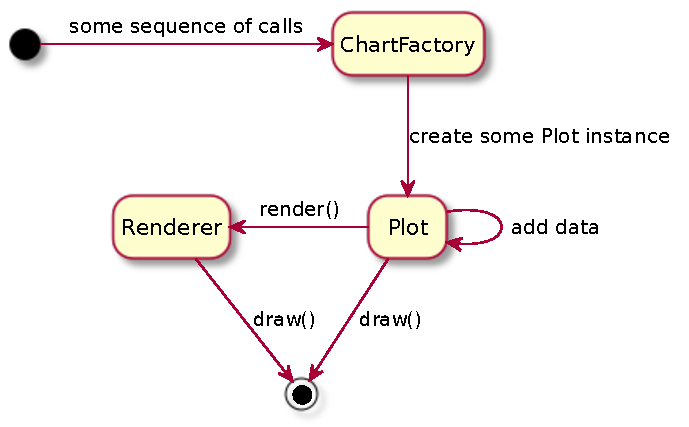
\includegraphics[width=0.5\textwidth]{pictures/draw-seq.pdf}
		\caption{A graphical representation of the main execution of calls required to draw a plot with data. Image created with \cite{plantuml}.}
		\label{fig:draw-seq}
	\end{figure}

	\textsl{Fig. \ref{fig:draw-seq}} is a representation of our understanding of the current code with respect to actually drawing/plotting some data. From our \texttt{main} function (the entrypoint of our system), there will be a sequence of calls resulting in us using the \textsf{Abstract Factory} design pattern from \texttt{JFreeChart}, located in the abstract \texttt{ChartFactory} class. Calling any of the create functions on this class, we will get an instance of a \texttt{Plot}. This can be any kind of \texttt{Plot}, as long as it is supported in \texttt{JFreeChart} and in the \texttt{ChartFactory}.
	
	Once we have obtained this \texttt{Plot}, we will probably add some data to it. This data comes in the form of the \texttt{Dataset} interface, which may or may not have been created already. Anyhow, assuming we have populated our \texttt{Plot}, we can now strive to display it.
	
	This will be done by calling the \texttt{draw} method on the \texttt{Plot} instance. In some cases, this function will automatically draw the plot, while in other classes, it first calls the internal (protected) \texttt{render} method. This \texttt{render} method in their turn will ask the renderer associated with this \texttt{Plot} to \texttt{draw} the data.

	\subsection{Design}
	\label{sec:design}
	Based upon the design we recovered, we can generate a new, better (and hopefully cleaner) design.
	
	First things first, we can see that all methods that extend from the \texttt{AbstractXYItemRenderer} implement the \texttt{XYItemRenderer} interface, that is also implemented by their base class. From the \textsf{Liskov Substitution Principle} \cite{Liskov94abehavioral} and the basic rules of inheritance, we know that it is not required for derived classes to also implement the interface that was implemented by the base class. Even stronger, we know that all of the functions that are required by this interface are implemented in the derived classes, because they are available in the base class. This is why we severed the implementation link of all classes that inherit from the \texttt{AbstractXYItemRenderer}.
	
	\begin{figure}[H]
		\centering
		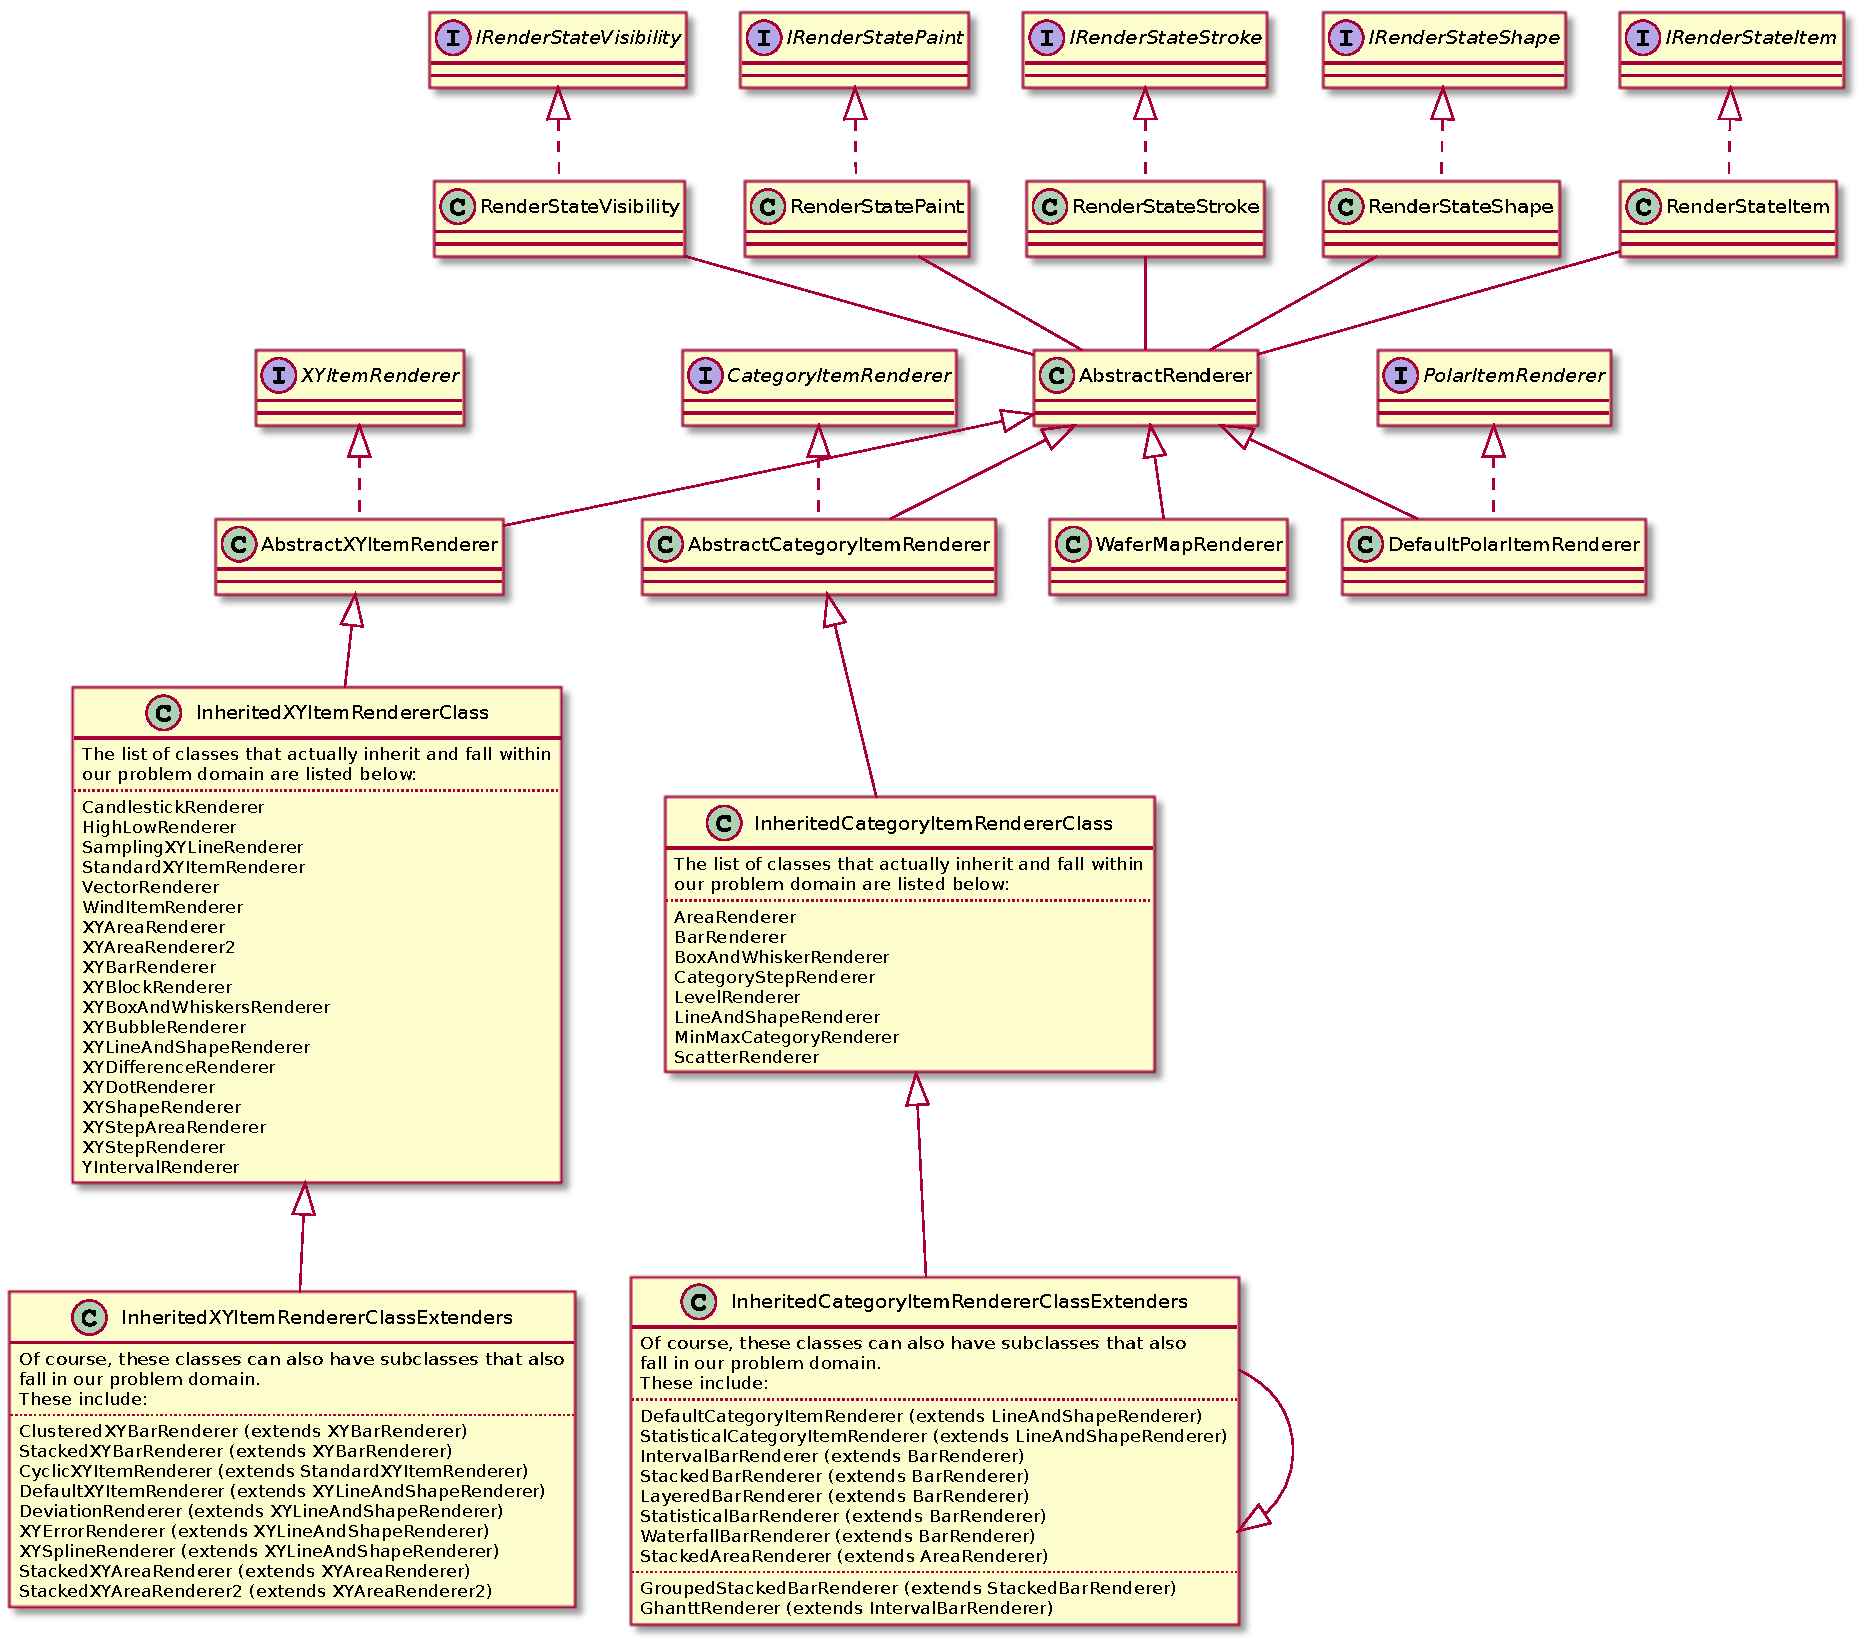
\includegraphics[width=\textwidth]{pictures/class-diagram-ours.pdf}
		\caption{An UML diagram, showing how we see the design. Image created with \cite{plantuml}. A bigger version can be found in \textsl{attachment \pageref{class-diagram-ours}}.}
		\label{fig:UML-ours}
	\end{figure}
	
	Unfortunately, without crowding too much of the class diagram, we didn't add all functions that are used in each class. If we would have done that, it would become clear that the \texttt{AbstractRenderer} is, in fact, a god class. \textsl{Split Up God Class} (9.3 from \cite{demeyer2009object}) tells us it is optimal to split up a class that holds too many functionalities, which is the case for the \texttt{AbstractRenderer}.
	
	From the comments in the code of the \texttt{AbstractRenderer}, we found that it had thirteen main functionalities, split up in sections: \texttt{Series Visibility}, \texttt{Series Visibility in Legend}, \texttt{Item Label Visibility}, \texttt{Paint}, \texttt{Fill Paint}, \texttt{Outline Paint}, \texttt{Item Label Paint}, \texttt{Stroke}, \texttt{Outline Stroke}, \texttt{Shape}, \texttt{Item Label Font}, \texttt{Positive Item Label Position} and \texttt{Negative Item Label Position}. Upon inspection, we found that not all extending classes used all these functions, which was an additional sign for us to split them up this way. We identified five categories from the original thirteen sections: \texttt{Visibility}, \texttt{Paint}, \texttt{Stroke}, \texttt{Shape} and \texttt{Item}. Each of these categories are identified with the \texttt{RenderState*}-classes and their respective interfaces.
	
	\subsection{Management}
	\label{sec:management2}
	\subsubsection{Actual Progress}
	As was mentioned in \textsl{section \ref{sec:original}}, we were not able to hold ourselves to the original planning of \textsl{Fig. \ref{fig:pert-orig}} and \textsl{Fig. \ref{fig:gantt-orig}}. This was mainly due to deadlines of other projects getting in the way and everything being due in the same week.
	
	\begin{figure}[H] 
		\centering 
		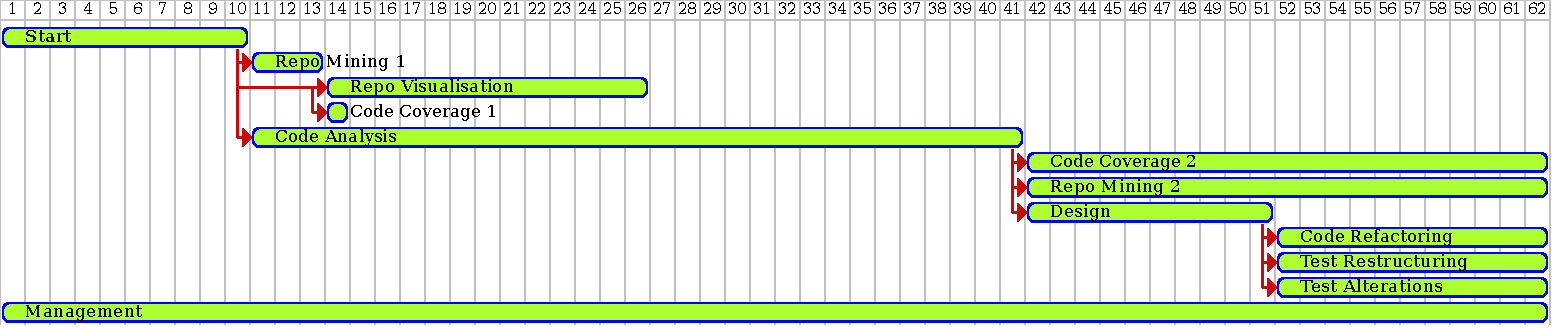
\includegraphics[width=\textwidth]{pictures/gantt-actual.pdf}
		\caption{Actual \textsf{Gantt} chart for the Refactoring of \texttt{JFreeChart}. Image made with \cite{plantuml}.} 
		\label{fig:gantt-actual} 
	\end{figure}

	The \textsf{Code Analysis} task was stretched thin over 31 days, allowing us to do a little bit here and there once we found the time. \textsl{Repo Mining} and \textsl{Code Coverage} were split into multiple tasks, the first around the deadline of the previous report and the second around the time of the actual \textsl{Design} phase.
	
	When looking back at the original \textsf{Gantt} chart, it's easy to identify a waterfall structure over the overall span of our project. And, besides the fact that this was an incredibly optimistic view on the project, we're glad we decided to work in an \textsf{Agile} manner for the actual refactoring. This way of working happened automatically, because we wanted to \textsl{Always have a Running Version} (7.5 from \cite{demeyer2009object}).
	
	This explains the recurrence of both the \textsl{Repo Mining} and \textsl{Code Coverage} tasks and also why, the second time they came around, these tasks span over the remainder of the project. At every new commit of main importance, we compared the new coverage and analyzed our repository again in \textsf{CodeScene}, making sure everything went as expected.
	
	Testing (both \textsl{Test Restructuring} and \textsl{Test Alterations}) went hand-in-hand with the \textsl{Code Refactoring} task. Because of our way of making sure that everything still worked and no tests failed (6.1, 6.3 and 7.6\footnote{\textsl{Test the Interface, not the Implementation} (6.4) also applies, mainly because this can be implicit due to refactoring. If we refactor some functionality and the tests keep working, they most definitely do not test the implementation.} from \cite{demeyer2009object}), some changes in the \textsl{Code Refactoring} also impacted these tasks.
	
	\subsubsection{Maintaining the Project}
	Of course, refactoring is not necessarily a guarantee for success. It has to be logical, sensible and maintainable long after the refactoring process is finished. The latter is definitely the case for our new design.
	
	The \texttt{AbstractRenderer} in our new design is no longer a God Class, but acts like a simple parent for all renderers. If you want to give them all some new functionality, you no longer have to search its previously massive file, but instead, you can add a new (or adapt an existing) \texttt{RenderState} class and/or interface. This way, all renderers became more modular and easier to maintain, while we \textsl{Conserve Familiarity} (7.11 from \cite{demeyer2009object}).
	
	\subsection{Refactoring}
	\label{sec:refactoring}
	The refactoring process itself can contain a lot of different aspects. As far as the \texttt{plot} package is concerned, we would have liked to \textsl{Transform Conditionals to Polymorphism} (10 from \cite{demeyer2009object}), but unfortunately for us, these patterns were not applicable\footnote{Which is a good thing for the official maintainers of \texttt{JFreeChart}.}. So instead, we tried to reduce the cyclomatic complexity of the \texttt{XYPlot} and the \texttt{CategoryPlot} classes.
	
	As for the \texttt{AbstractRenderer}, we explained earlier in this document (see \textsl{section \ref{sec:design}}) how we could refactor this class.
	
	\section{Preserved Behaviour}
	\label{sec:pb}
	Of course, in order to be able to say that our refactoring process was effective, we must compare our results to the original source code. While tools like \textsf{iClones} \cite{iclones} automatically come bundled with a version comparison, others, unfortunately, do not. This is why, for this phase of the project, we decided to jump back and forth to the original version of our project and bundle all of our findings below.
	
	\subsection{Test Coverage (Cobertura)}
	As we described in \textsl{section \ref{sec:coco}}, we've been using the tests from \texttt{JFreeChart}. As you can see, our project still passes on all of them, meaning that we (at least) provide the same functionality as when we started (6.1 and 7.6 from \cite{demeyer2009object}).
	
	Taking a look at the code coverage reports from \textsf{Cobertura}, we can clearly see that we have some subtle differences. These changes can be either positive (the percentages went up) or negative (they went down). See \textsl{attachments \pageref{cobertura-begin} and \pageref{cobertura-now}}.
	
	For the positive changes in these reports, we know they are a good thing. Generally, this implies the refactoring we've done caused the tests to cover more code, giving us the information that there is more code that has passed the tests.
	
	The negative changes on the other hand can also be seen as favorable. The main reason for this is because we removed some lines of code from these files and placed them elsewhere, while the existing covered functionality remained.
	
	\subsection{Hotspots (CodeScene)}
	At the beginning of our project, \textsf{CodeScene} gave us about 5 percent in \textsl{Red Hotspots}. These refer to the complexity of the code, internal coupling, refactoring targets... Our refactoring process allowed this number to drop to about 2.8\%.
	
	This means that, even though we now have some \textsl{High-Risk Commits}, our refactored project is overall better and cleaner designed.
	
	As said previously (in \textsl{section \ref{sec:refactoring}}), we tried our best in reducing the overall cyclomatic complexity of the project (mainly the \texttt{plot} package). But for the most part, this isn't the way to go. Refactoring because of refactoring is bad practice if it doesn't optimize the overall structure of the system.
	
	This is why we went looking for duplicate code and features that could be extracted to other places. Overall, we tried to reduce the complexity and coupling of the original system.
	
	When comparing \textsl{attachment \pageref{refactoring-package-plot}} to \textsl{attachment \pageref{refactoring-package-plot-ours}}, you can clearly see that more classes are identified as refactoring targets. Seeing as we did not change any code in these classes, we deduce that \textsf{CodeScene} identifies these targets percentage-wise and that our overall percentage must have dropped. The same can be said when comparing the overviews of both the refactoring targets (\textsl{attachment \pageref{refactoring-overview}} to \textsl{attachment \pageref{refactoring-overview-ours}}) and the hotspots (\textsl{attachment \pageref{hotspots-overview}} to \textsl{attachment \pageref{hotspots-overview-ours}}). Although, in the latter comparison, we clearly have smaller orbs to compare, meaning the hotspot-percentage went down.
	
	In \textsl{attachment \pageref{refactoring-package-renderer-ours}}, you can find that the \texttt{AbstractRenderer} is a refactoring target no more.
	
	\subsection{Code Smells (SonarQube)}
	As discussed in \textsl{section \ref{sec:sonarqube}}, we tried identifying our code smells using \textsf{SonarQube}. When we take a look at the general results (which can be seen in \textsl{attachment \pageref{sonarcloud-orig}}) and lay them next to those of our new system (as in \textsl{attachement \pageref{sonarcloud}}), we see our debt\footnote{The estimated time to fix all code smells.} and our duplication percentage went down.
	
	As for all other metrics, those all remained the same, a sign that we purely redesigned our system instead of us trying to fix all issues.
	
	
	\section{Further Work}
	As with any software project, it is perfectly possible to keep on being fixated on small, unimportant details. This is why it is important to retain a clear image of the problem at hand (see \textsl{section \ref{sec:pah}}).
	
	The main focus of this project was to refactor so that the feature of allowing each point to have another shape can be easily implemented. Thus, we focused our attention on the \texttt{AbstractRenderer} and \texttt{plot} package, but there is more to \texttt{JFreeChart}. Possible further work includes the refactoring of other aspects of the code, so there are more features to be added easily.

	\clearpage
	\bibliographystyle{plain}
	\bibliography{references}
	
	\section*{Attachments}
	On the following pages, we've included a set of screenshots from \textsf{CodeScene} that are referred to in the previous sections. The attachment number is overlayed over the image.
	
	\clearpage
	\setcounter{page}{1}
	
	\attachment{cobertura-begin}
	\attachment{cobertura-now}
	
	\attachmentpdf{class-diagram-begin}
	\attachmentpdf{class-diagram-ours}
	
	\attachment{intellij-plugins}
	
	\attachment{sonarcloud-orig}
	\attachment{sonarcloud}
	
	\attachment{hotspots-overview}
	\attachment{hotspots-package-renderer}
	\attachment{hotspots-package-plot}
	\attachment{refactoring-overview}
	\attachment{refactoring-package-plot}
	\attachment{refactoring-list}
	\attachment{refactoring-XYPlot}
	\attachment{refactoring-CategoryPlot}
	\attachment{refactoring-PiePlot}
	\attachment{refactoring-AbstractXYItemRenderer}
	\attachment{refactoring-AbstractCategoryItemRenderer}

	\attachment{hotspots-overview-ours}
	\attachment{hotspots-package-renderer-ours}
	\attachment{refactoring-overview-ours}
	\attachment{refactoring-package-plot-ours}
	\attachment{refactoring-package-renderer-ours}
	
\end{document}